\documentclass[./main.tex]{subfiles}
\graphicspath{{\subfix{./images/}}}

\begin{document}

Arrays are data structures\footnote{A structure by which you can store data!} whereby you can store lists of information. The cats in your house or the people, a row of tall lockers and the names of their owners, or a list of data you need to sort.

\subsection{Important Information}

In pseudocode:

\begin{itemize}
    \item Arrays in pseudocode are \textbf{\emph{static}}. This means that the length \emph{cannot change}. No appending, no removing, etc.
    \item You must declare the beginning and end of the array. All the values will be set to uninitialized; i.e. invalid.
    \item You can freely index any element despite if it is initialized or not and write to it.
\end{itemize}

and in Python:

\begin{itemize}
    \item They are called lists\footnote{There are arrays that behave like pseudocode arrays in Python in a library; but please do not use them. They are archaic, primitive and provide no benefit over lists.}.
    \item They are dynamic, meaning you can change the length of the array. You can add items after the end to change the length and remove them.
    \item You do not need to and in fact cannot declare the beginning and end of the list.
    \item You cannot freely index any element. It must be initialized first, or at least be set to {\ccmono None}.
\end{itemize}

\textbf{NOTE: I will refer to arrays and lists as the same thing in pseudocode, interchangeably.}

\subsection{1D arrays}

\subsubsection{Declaration, Indexing, and Population}

Declaring an array is trivial:

\begin{minted}{text}
DECLARE <variable>:ARRAY[<begin>:<end>] OF <type>
\end{minted}

And as an example:

\begin{minted}{text}
// I want 3 cats, so I give space for elements between 1 and 3.
DECLARE CatNames:ARRAY[1:3] OF STRING 

DECLARE Scores:ARRAY[1:8] OF INTEGER
\end{minted}

When you work with arrays, you also have to access the data stored within them. This process is known as \emph{indexing}.

\begin{figure}[h]
    \centering
    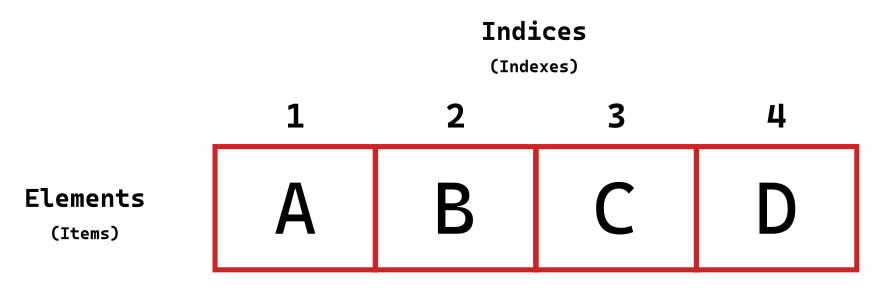
\includegraphics[width=0.8\textwidth]{arrays.png}
    \caption{A breakdown and representation of an array.}
    \label{fig:arrays}
\end{figure}

In figure \ref{fig:arrays}, the index is the nth element. Indices in other languages like Python begin at 0, and for a very good reason\footnote{Advanced learners: this is due to its heritage in older languages like C. Arrays are actually not values that stand by themselves, as the size isnt promised to be some value. Attempting to remove/modify the array will cause memory to overlap, which is very bad. Instead, an array is simply a \emph{location in memory where data is}. The location in memory will have the array's data; uniformly sized data that are equally spaced out. Therefore, if you were to get the first item of a list at address 4000, the first item would be 4000+0. However, the second one would be 1 address away, so 4000+1, then 4000+2, etc. This is why arrays begin at 0; it is simply the \emph{offset} from the beginning of the memory address.}. However, you just need to remember that indices start at 1 in pseudocode.

To index that array (let's call it {\ccmono Array}), one may write {\ccmono Array[<index>]}. In code, it looks like

\begin{minted}{text}
OUTPUT Array[2] // gets the second item in the array.
\end{minted}

In fact, you may also write to the array this way:

\begin{minted}{text}
Array[2] <- 'F' // sets the second element to the character F.
\end{minted}

To wrap this new knowledge up, let us create an array of food items.

\begin{minted}{text}
DECLARE FoodItems:ARRAY[1:5] OF STRING
\end{minted}

We must fill it up with items. In programming terms, this is known as \emph{populating}.

\begin{minted}{text}
FoodItems[1] <- "Burger"
FoodItems[2] <- "Chilli Crab"
FoodItems[3] <- "Paneer Tikka"
FoodItems[4] <- "Fried Rice"
FoodItems[5] <- "Beans on Toast"
\end{minted}

Now, there are items in the list and we can freely index it now!

\subsubsection{Iterating through an array}

Revisit section \ref{sec:for_loops} on for loops.

\begin{minted}{text}
FOR Counter <- 1 TO 5
    OUTPUT Counter
NEXT Counter
\end{minted}

For loops allow us to count through values between 1 and something. Conveniently, array indexes are numbers. \textbf{Do you see the pattern?}

\textbf{YES! We can use for loops to go through the items in a list!}

\begin{minted}{text}
FOR Counter <- 1 TO 5 // our list is 5 items long
    OUTPUT FoodItems[Counter]
NEXT Counter
\end{minted}

Will output:

\begin{minted}{text}
Burger
Chilli Crab
Paneer Tikka
Fried Rice
Beans on Toast
\end{minted}

Armed with this information, let us practice.

\newpage
\subsubsection{Exercises}

Write pseudocode for all below questions.

\begin{enumerate}
    \item With the array we declared before, loop through it backwards and print {\ccmono Do you like <the food item>?}
        \mediumlines
    \item Create a constant {\ccmono FoodsLength} and set it to 10. Create a new array {\ccmono FoodsLength} items long called {\ccmono FavoriteFoods}.
        \mediumlines
    \item Move all the items in the old array to the new array, without copying the values directly. Only use indexing to move the values.
        \mediumlines
    \item Redo question 3, but you may not write more than 3 lines. Use the correct loop for this.
        \mediumlines
    \item In the most logical and optimized manner, ask the user to populate the 6th to the 10th index in the new array through user input and a loop of your choosing. Do not write more than 1 input statement. \emph{hint: counters and indexing!}
        \largelines
    \item Iterate through your new list and print out each of the items in the list. 
        \largelines
\end{enumerate}

\end{document}
